\documentclass[12pt,a4paper]{article}
\usepackage[UTF8]{ctex}
\usepackage{geometry}
\usepackage{graphicx}
\usepackage{float}
\usepackage{amsmath}
\usepackage{amsfonts}
\usepackage{amssymb}
\usepackage{booktabs}
\usepackage{multirow}
\usepackage{array}
\usepackage{longtable}
\usepackage{enumerate}
\usepackage{fancyhdr}
\usepackage{lastpage}
\usepackage{hyperref}

% 页面设置
\geometry{left=2.5cm,right=2.5cm,top=2.5cm,bottom=2.5cm}

% 页眉页脚设置
\pagestyle{fancy}
\fancyhf{}
\fancyhead[C]{实\hspace{0.5em}验\hspace{0.5em}报\hspace{0.5em}告}


% 标题设置


\begin{document}

% 正文第一行标题
\noindent
{\Large \textbf{实验七：}\underline{\textbf{示波器和函数发生器的使用}}} \hfill {\Large \textbf{实验成绩：}\underline{\hspace{3cm}}}
\vspace{0.5cm}

\section*{一、实验目的}
\begin{enumerate}
    \item 熟悉示波器和信号发生器的主要开关、旋钮的使用方法。
    \item 学习示波器屏幕菜单的操作方法。
    \item 掌握用示波器测量电压与时间的方法。
\end{enumerate}

\section*{二、实验原理}
\begin{enumerate}
    \item 示波器是现代测量中常用的仪器之一，可分为模拟示波器和数字示波器。示波器可看作功能强大的电压表，测量精度高，测量速度快，具备高速存储能力。它主要用于电压波形的测量，但是只能测量电路参考点与被测点之间的电压。
    \item 信号发生器是一种可产生多种波形、不同频率、不同幅值的信号源设备。
    \item 信号发生器在实验中担任输入信号源的任务，可产生实验所需的各种波形和频率；示波器在实验中用作波形观测和参数测量仪器。

\end{enumerate}

\section*{三、思考题}
\begin{enumerate}
    \item 示波器输入端的"交流"(AC)、"直流"(DC)、"接地"耦合方式分别表示什么含义？
    
    解：

    (1) AC交流耦合：阻止直流分量通过，只允许交流分量进入示波器，适用于测量交流信号或含有直流偏置的交流信号的交流部分。

    (2) DC直流耦合：允许直流和交流分量都通过，能够显示信号的真实波形包括直流偏置，适用于测量包含直流分量的信号。

    (3) 接地(GND)耦合：将输入端接地，显示零电位基准线，用于确定示波器显示屏上的零电位位置。
    
    \item 垂直灵敏度、水平扫描速度分别表示什么含义？如何调整其大小？
    
    解：

    (1) 垂直灵敏度(V/div或mV/div)：表示屏幕上每个垂直格对应的电压值，决定了电压测量的精度和波形的垂直显示范围。通过旋转垂直灵敏度旋钮按5-2-1序列调节(如5V/div→2V/div→1V/div→500mV/div...)。

    (2) 水平扫描速度(s/div、ms/div或μs/div)：表示屏幕上每个水平格对应的时间值，决定了时间测量精度和波形的水平显示范围。通过旋转水平扫描速度旋钮按4-2-1序列调节。
    
    \item 示波器水平和垂直控制钮中的"位置"(position)旋钮的作用是什么？
    
    解：

    (1) 垂直位置旋钮：用于调节波形在屏幕上的垂直位置，可以将波形上下移动到合适的显示位置，便于观察和测量，不改变信号的幅值大小。

    (2) 水平位置旋钮：用于调节波形在屏幕上的水平位置，可以将波形左右移动，选择观察信号的不同时间段，便于分析信号的特定部分，不改变信号的时间关系。
    
    \item 测量一个$u_{\text{p-p}}=2\text{V}$的信号，如要使其在显示屏的垂直方向上尽可能大，但又不能超出显示屏的有效位置，则Y轴灵敏度开关应放在什么位置？
    
    解：
    
    Y轴灵敏度开关应设置在500mV/div位置。因为示波器屏幕通常有8个垂直格，当设置为500mV/div时，屏幕可显示的最大电压范围为8×500mV=4V。对于峰峰值为2V的信号，正好可以充分利用显示屏的垂直空间(占用4格)，既能最大化显示又不会超出屏幕范围。
    
    \item 要测量一个$f=100\text{Hz}$的信号，如果要求信号在水平方向上显示两个周期的波形，则示波器水平分辨率应调至多少？
    
    解：
    
    水平分辨率应设置在2ms/div。计算过程：$f=100\text{Hz}$的信号周期$T=\frac{1}{f}=\frac{1}{100}=10\text{ms}$，两个周期的时间为$2T=20\text{ms}$。示波器屏幕通常有10个水平格，要显示20ms的信号，每格应对应$\frac{20\text{ms}}{10}=2\text{ms}$，因此水平分辨率应设置为2ms/div。
    
    \item 何为示波器的Y-T显示方式和X-Y显示方式？
    
    解：

    (1) Y-T显示方式：纵坐标(Y)表示电压幅值，横坐标(T)表示时间，是示波器的标准显示模式。适用于观察信号随时间的变化情况，测量信号的幅值、频率、周期、相位等参数。

    (2) X-Y显示方式：将两个输入信号分别作为横坐标(X)和纵坐标(Y)，显示两信号间的相互关系轨迹。适用于测量两信号间的相位关系、频率比较、李萨如图形分析等，常用于相位差测量和频率比较。
\end{enumerate}


\section*{四、实验任务与线路}
\begin{enumerate}
    \item 信号发生器操作：选定适当的波形类型和CH1信号通道，调节频率、幅值、偏置电压等参数。对于正弦波，可调节频率和幅值；对于方波，可调节频率、幅值、偏置量和占空比，注意Output输出开关的状态。
    \item 示波器的触发功能：触发功能可以捕获并稳定显示连续的信号波形。触发器包括触发电平、触发斜率、触发源等设置。对于周期性信号，使用自动触发；对于单次信号，使用单次触发。Autoset自动设置功能可根据输入信号自动调节合适的显示参数。
    \item 波形显示调节：包括波形的水平位置调节和垂直位置调节。耦合方式有交流耦合、直流耦合和接地方式。使用Acquire菜单可调出采集设置，可在YT扫描和XY显示模式间切换。其中垂直灵敏度（V/div，mV/div）按 5-2-1序列调节；水平扫描速度分级为 4-2-1序列调节。

\begin{figure}[H]
    \centering
    
\includegraphics[width=0.8\textwidth]{E7_preview/schematic.png}
    \caption{实验线路图}
    \label{fig:schematic}
\end{figure}
\end{enumerate}

\section*{五、实验数据记录与分析}
\subsection*{实验一}

\begin{enumerate}
    \item 同一坐标系下绘制 CH1、CH2 两条扫描线
        \begin{figure}[H]
        \centering
        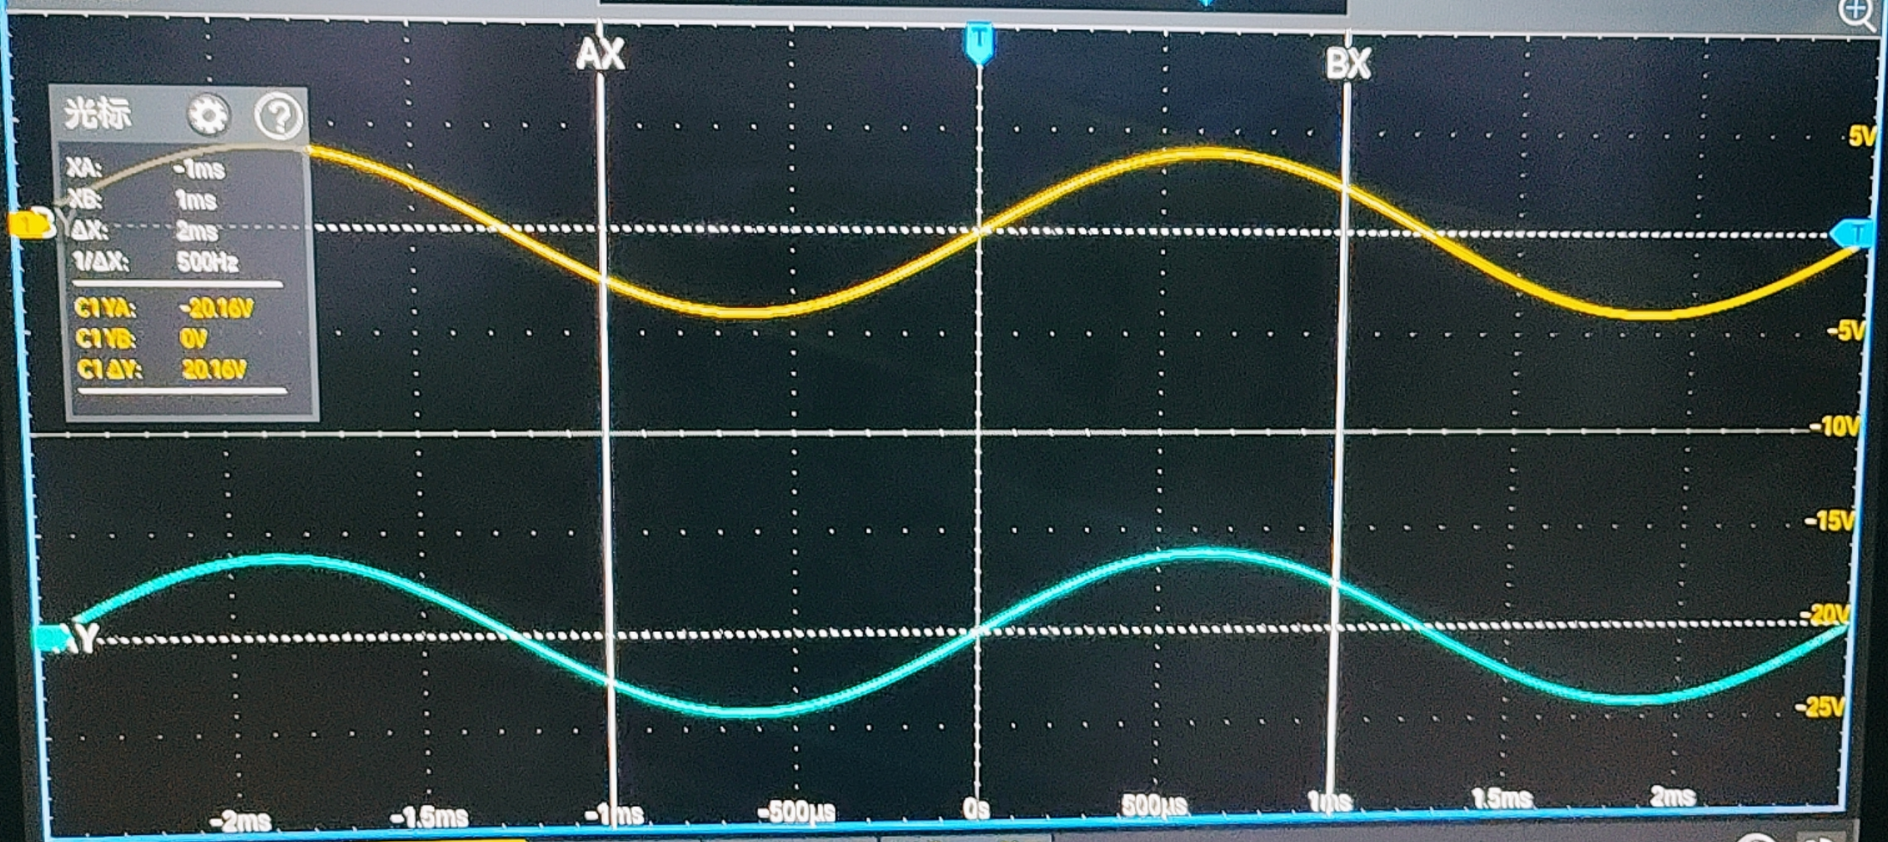
\includegraphics[width=0.8\textwidth]{E7/CH1_CH2两条扫描线.png}
        \caption{同一坐标系下绘制 CH1、CH2 两条扫描线}
        \label{fig:1}
        \end{figure}
    \item 同一坐标系下绘制 CH1、CH2 两个波形
        \begin{figure}[H]
        \centering
        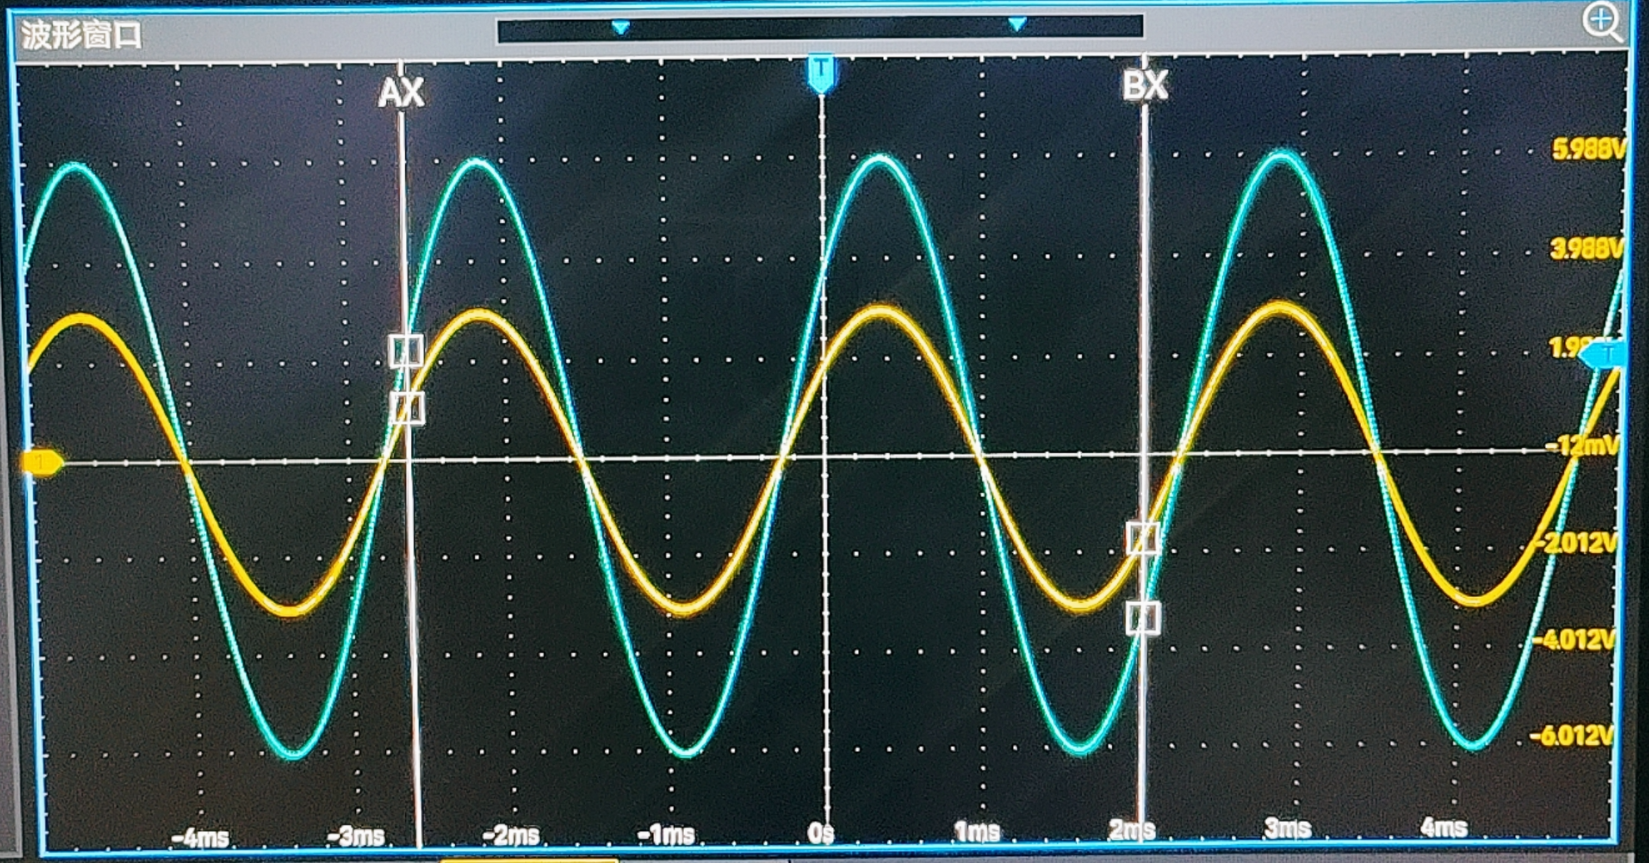
\includegraphics[width=0.8\textwidth]{E7/CH1_CH2两个波形.png}
        \caption{同一坐标系下绘制 CH1、CH2 两个波形}
        \label{fig:2}
        \end{figure}
    \item 绘制 XY 坐标系下的波形
        \begin{figure}[H]
        \centering
        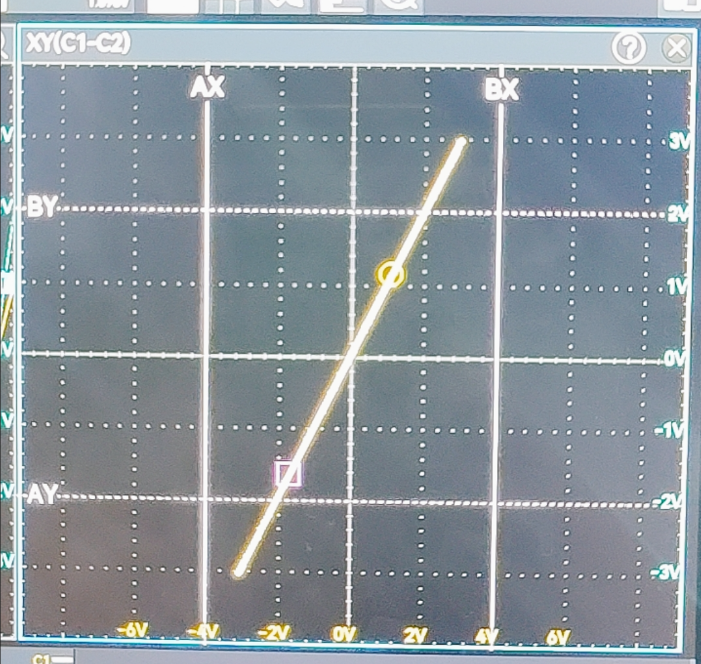
\includegraphics[width=0.8\textwidth]{E7/XY坐标系下的波形.png}
        \caption{XY 坐标系下的波形}
        \label{fig:3}
        \end{figure}
    \item 分别绘制不同扫描速度下的波形
        \begin{figure}[H]
        \centering
        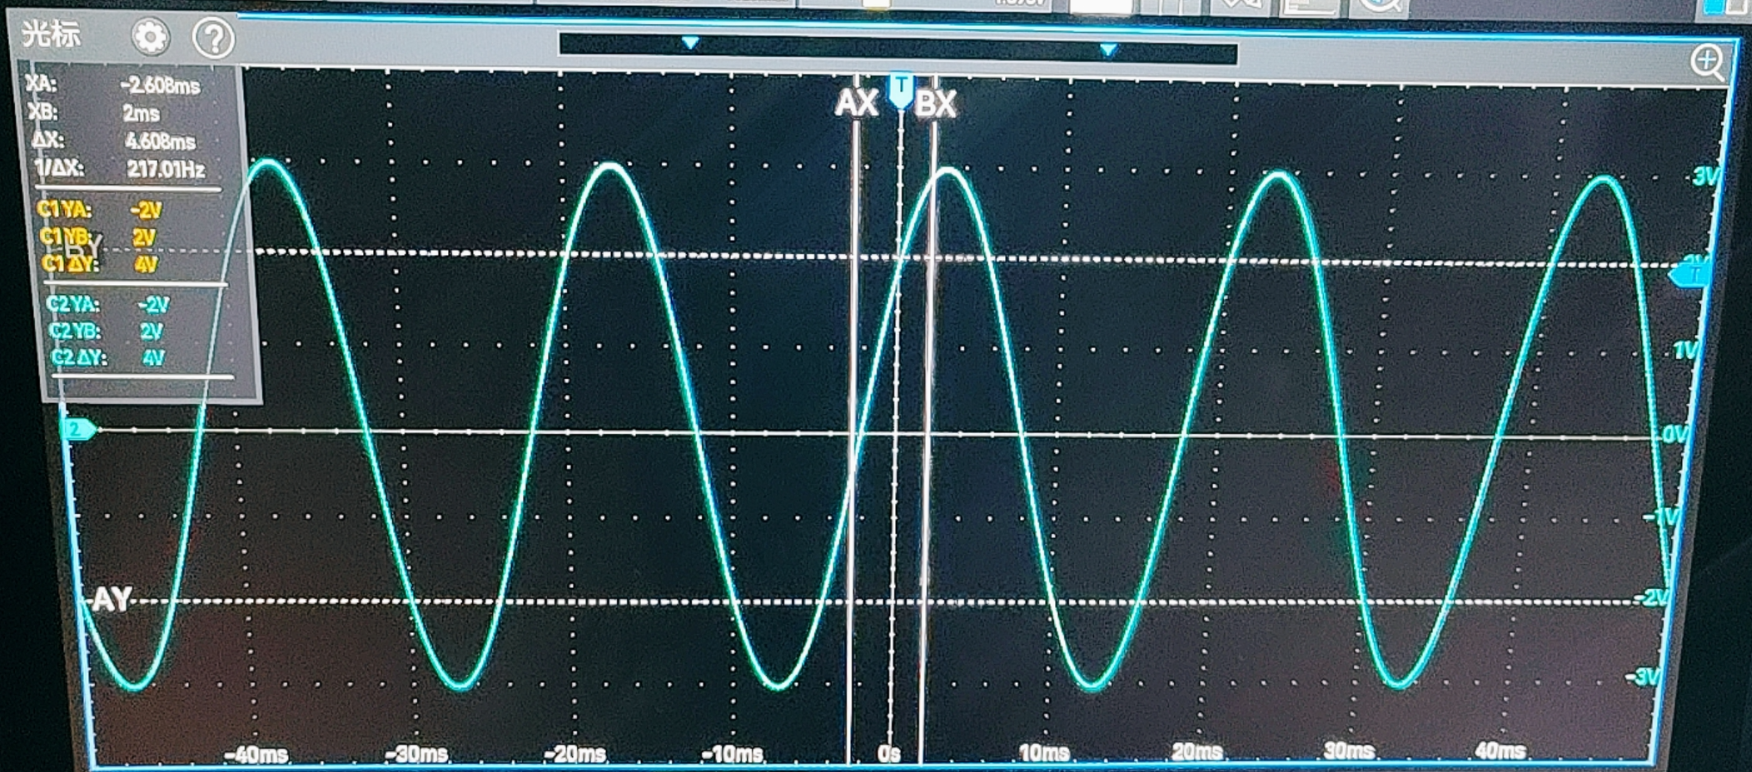
\includegraphics[width=0.8\textwidth]{E7/不同扫描速度下的波形_1.png}
        \caption{水平扫描速度10ms/div下的波形}
        \label{fig:4-1}
        \end{figure}
        \begin{figure}[H]
        \centering
        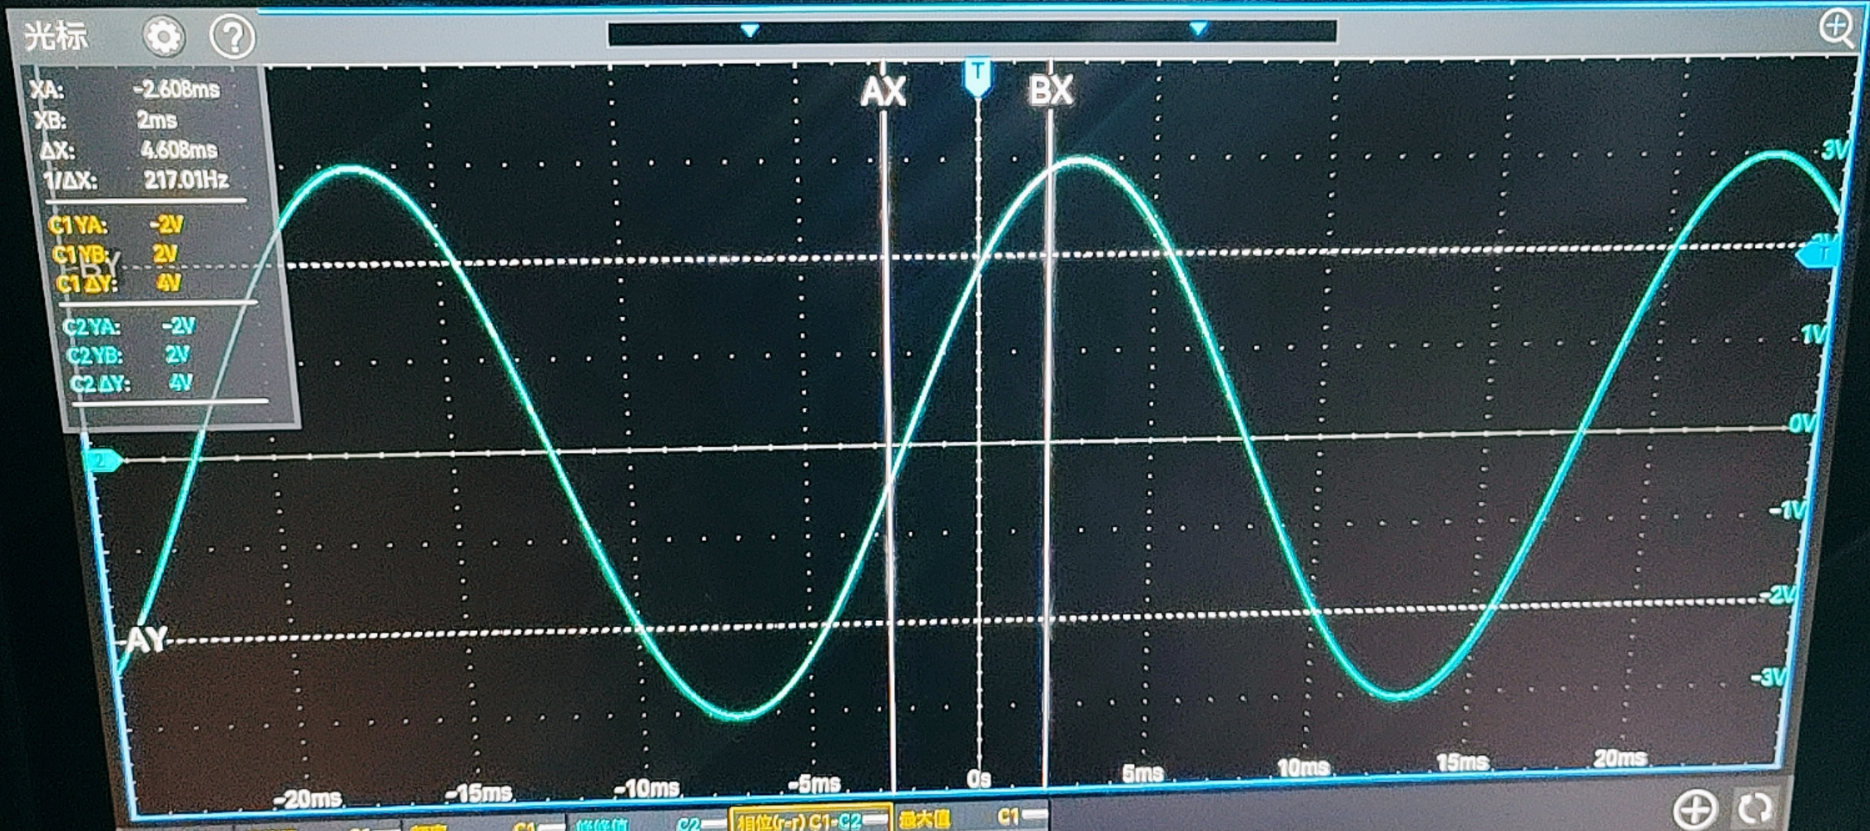
\includegraphics[width=0.8\textwidth]{E7/不同扫描速度下的波形_2.png}
        \caption{水平扫描速度5ms/div下的波形}
        \label{fig:4-2}
        \end{figure}
    \item 同一坐标系下绘制 CH1、CH2、CH3 三个波形
        \begin{figure}[H]
        \centering
        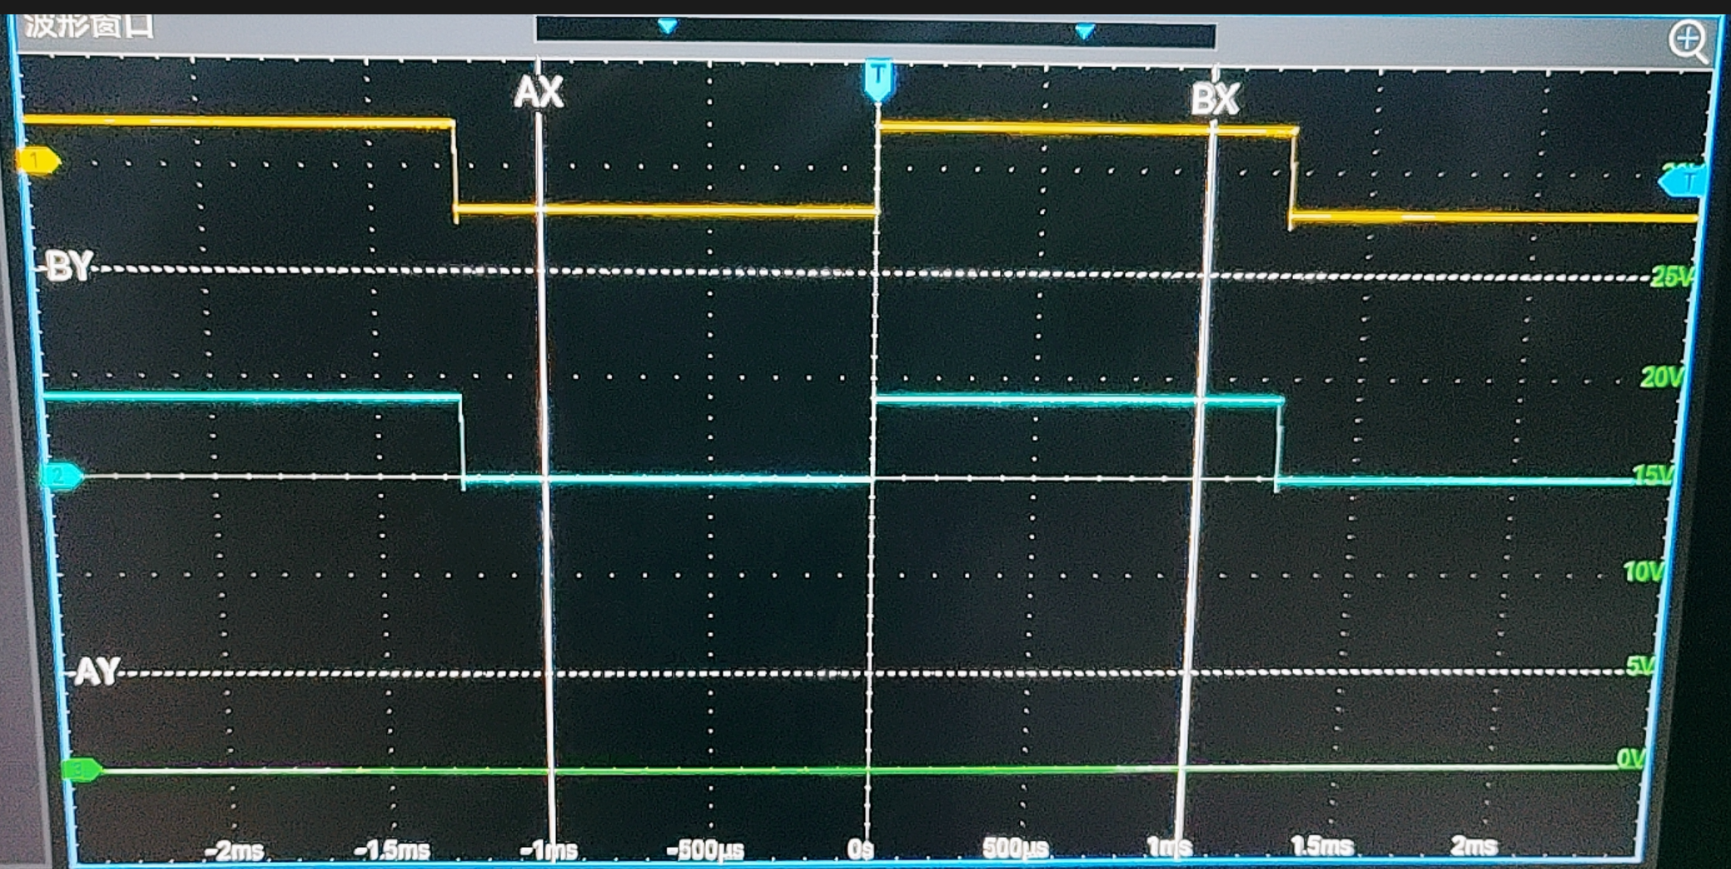
\includegraphics[width=0.8\textwidth]{E7/CH1CH2CH3三个波形.png}
        \caption{同一坐标系下绘制 CH1、CH2、CH3 三个波形}
        \label{fig:5}
        \end{figure}
\end{enumerate}

\subsection*{实验二}
\begin{enumerate}
    \item 负载为$R=200\Omega$时的波形图
        \begin{figure}[H]
        \centering
        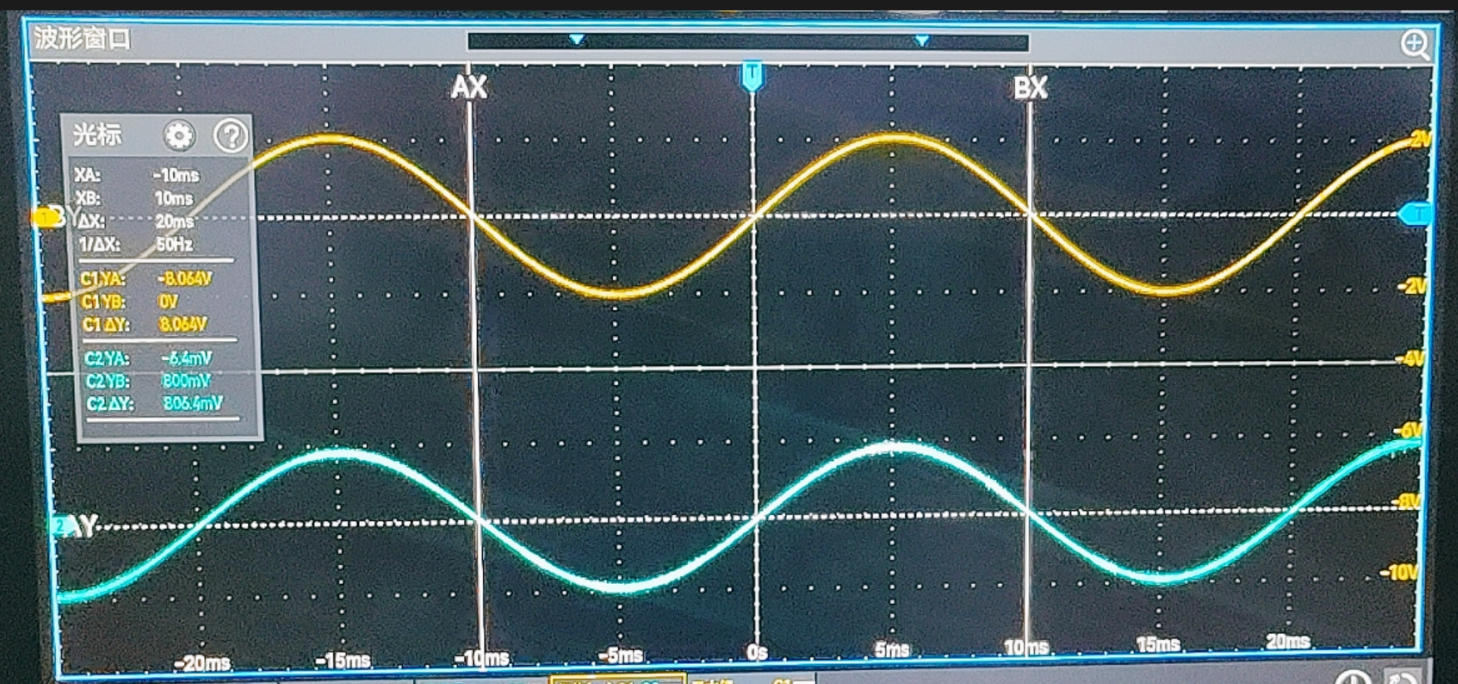
\includegraphics[width=0.8\textwidth]{E7/R.png}
        \caption{负载为$R=200\Omega$时的波形图
        \label{fig:R}
        }
        \end{figure}
    \item 负载为$C=2.2\mu F$时的波形图
        \begin{figure}[H]
        \centering
        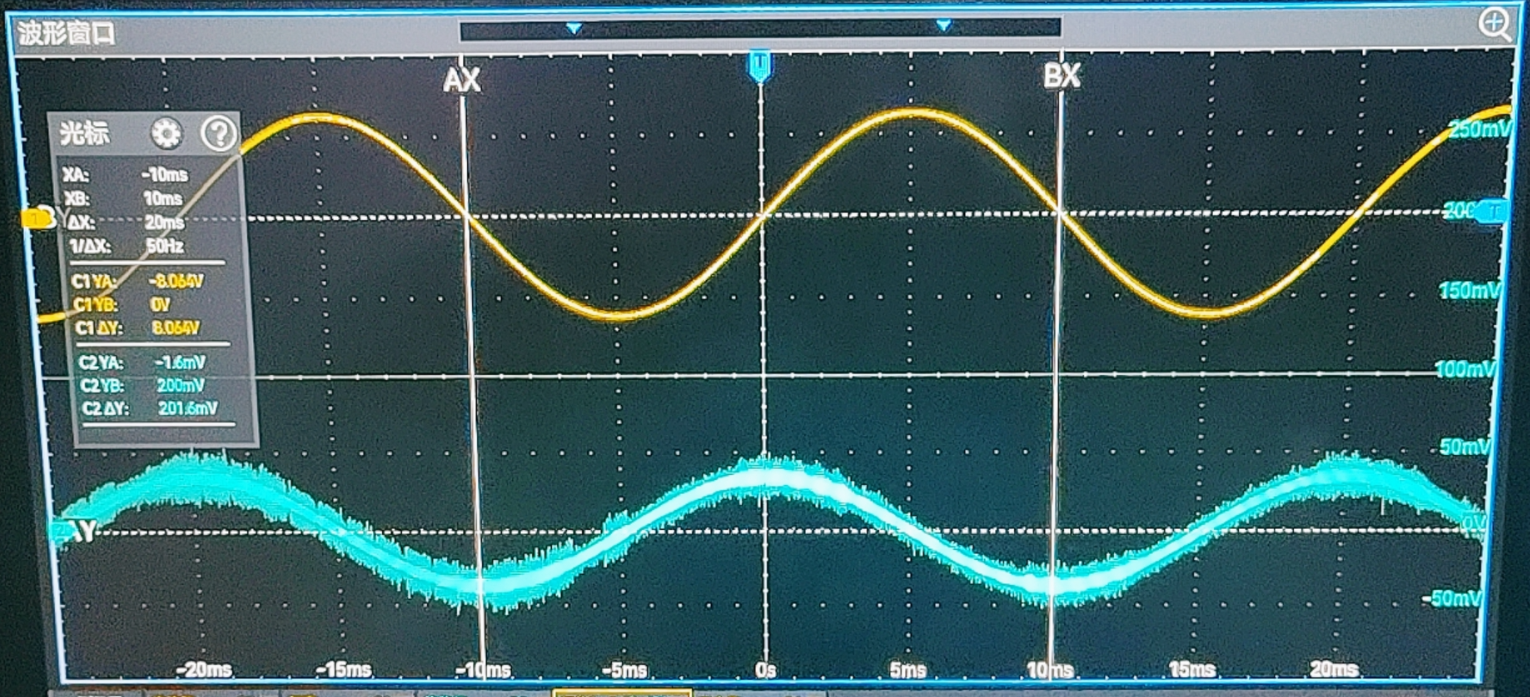
\includegraphics[width=0.8\textwidth]{E7/C.png}
        \caption{负载为$C=2.2\mu F$时的波形图
        \label{fig:C}
        }
        \end{figure}
    \item 负载为$L=100mH$时的波形图
        \begin{figure}[H]
        \centering
        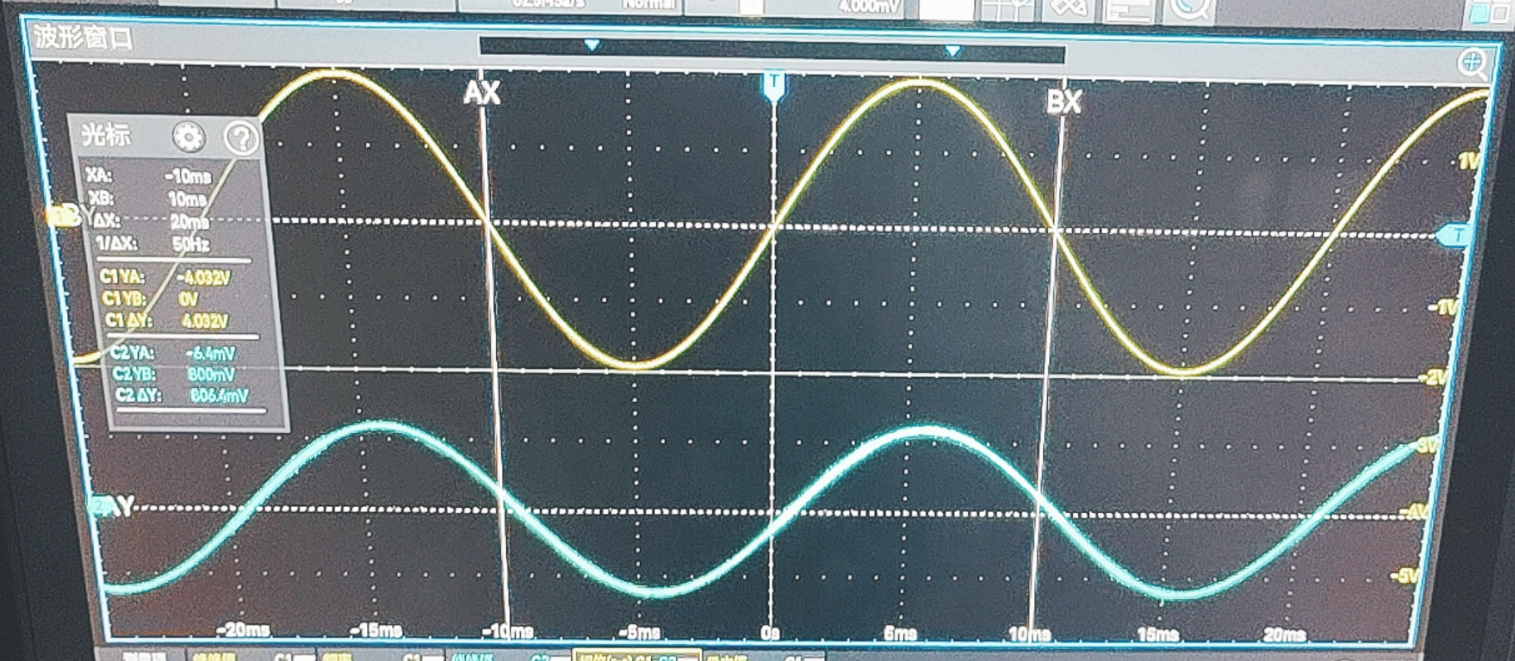
\includegraphics[width=0.8\textwidth]{E7/L.png}
        \caption{负载为$L=100mH$时的波形图
        \label{fig:L}
        }
        \end{figure}
\end{enumerate}

\section*{六、实验小结}
通过本次实验，我熟悉了示波器和信号发生器的基本操作方法，掌握了如何调节示波器的垂直灵敏度和水平扫描速度，以及如何使用示波器的触发功能来稳定显示波形。通过测量不同负载下的电压和电流关系，我加深了对电路中电阻、电容和电感元件特性的理解。此外，实验过程中遇到了一些挑战，如调整波形显示位置和选择合适的触发模式，但通过反复尝试和调整，最终成功解决了这些问题。总体而言，这次实验不仅提升了我的动手能力，也增强了我对电子测量仪器的认识，为今后的学习和研究打下了坚实的基础。


\end{document}

